\chapter{Multiplicity properties of the Galactic WNL population}\label{ch:wnl}

\textit{The work presented in this chapter is based on:}

\textbf{A spectroscopic multiplicity survey of Galactic Wolf-Rayet stars: III. The northern WNL sequence}

\textbf{K. Dsilva}, T. Shenar, H. Sana and P. Marchant

Soon to be submitted to {\sc Astronomy and Astrophysics}.

\textbf{Author contributions:} K. Dsilva performed the data reduction and computed the radial velocities in this chapter with the guidance of H. Sana and T. Shenar. The Monte-Carlo simulations were run by H. Sana. The Bayesian framework was developed by P. Marchant and H. Sana. All the authors assisted with the evolutionary interpretations of the presented results and contributed significantly to the text, which was written by K. Dsilva.
\newpage

\begin{abs}
\vspace{3mm}
\textbf{Original abstract:}
\newline \newline
Massive stars are powerful cosmic engines that have a huge impact on their surroundings and host galaxies. The majority of massive stars will interact with a companion star during their evolution. The effects of this interaction on their end-of-life products are currently poorly constrained. In the phases immediately preceding core-collapse, massive stars in the Galaxy with $M_i \gtrsim 20$ may appear as classical Wolf-Rayet (WR) stars. The multiplicity properties of the WR population are thus required to further our understanding of stellar evolution at the upper-mass end.
  % aims heading (mandatory)
As the final contribution of a homogeneous radial velocity (RV) survey, this work aims to constrain the multiplicity properties of northern, Galactic, late-type nitrogen-rich Wolf-Rayet (WNL) stars. We compare their intrinsic binary fraction and orbital period distribution to the carbon-rich (WC) and early-type nitrogen-rich (WNE) WR populations from previous works.
% methods heading (mandatory)

We obtained high-resolution spectra of the complete magnitude-limited sample of 11 Galactic WNL stars with the Mercator telescope on the island of La Palma. We used cross-correlation with a log-likelihood framework to measure relative RVs and flagged binary candidates based on the peak-to-peak RV dispersion. By using Monte-Carlo sampling and a Bayesian framework, we computed the three-dimensional likelihood and one-dimensional posteriors for the upper period cut-off (\logPmaxWNL{}), power-law index (\piWNL{}) and intrinsic binary fraction (\fintWNL{}).
% results heading (mandatory)

Adopting a threshold $C$ of 50\,\kms{}, we derived \fobsWNL{}$\,=\,0.36\,\pm\,0.15$. Our Bayesian analysis produces \fintWNL{}$\,=\,0.42\substack{+0.15 \\ -0.17}$, \piWNL{}$\,=\,-0.70\substack{+0.73 \\ -1.02}$ and \logPmaxWNL$\,=\,4.90\substack{+0.09 \\ -3.40}$ for the parent WNL population. The combined analysis of the Galactic WN population results in \fintWN{}$\,=\,0.52\substack{+0.14 \\ -0.12}$, \piWN{}$\,=\,-0.99\substack{+0.57 \\ -0.50}$ and \logPmaxWN$\,=\,4.99\substack{+0.00 \\ -1.11}$. The observed period distribution of reported orbital periods of Galactic WN and WC binaries is in agreement with these results.
% conclusions heading (optional), leave it empty if necessary
The period distribution of Galactic WN binaries peaks at $P{\sim}1-10\,$d while that of the WC population at $P{\sim}5000\,$d, a shift that cannot be reconciled by orbital evolution due to mass loss or mass transfer.
At long periods, the evolutionary sequence O\,($\xrightarrow{}$LBV)\,$\xrightarrow{}$\,WN$\xrightarrow{}$WC seems feasible. The high frequency of short-period WN binaries compared to WC binaries suggests that they either tend to merge, or that the WN components in such binaries rarely evolve into WC stars in the Galaxy.
\end{abs}


\section{Introduction}

% Classical WN stars with very thick, dense winds can appear as WNL stars. However, very-massive main-sequence stars can also appear as WNL sub-types.

Late-type Wolf-Rayet stars of the nitrogen sequence (WNL) stars can either be classical (hydrogen-depleted, post main sequence) or very-massive main sequence (hydrogen burning) stars. It is challenging to differentiate between the two, although the main-sequence WNL stars are generally more luminous (and more massive) than classical WNL stars \citep{hamann_galactic_2019}. In this chapter, we focus on the analysis of the remaining 11 WNL stars in our sample. We find that the multiplicity properties of the WNL population are consistent with the WNE population from Chapter \ref{ch:wne}, and so we perform a combined analysis by comparing the multiplicity properties of the Galactic WN population to those of the WC population from Chapter \ref{ch:wc}. The sample, data reduction and normalisation are briefly explained in Sect. \ref{sect:sample_WNL}. The RV analysis is discussed in Sect. \ref{sect:rv_WNL}. Our results are presented in Sect. \ref{sect:results_WNL} and discussion in Sect. \ref{sect:discussion_WNL}. We present our conclusions in Sect. \ref{sect:conclusions_WNL}.


\section{Sample and data reduction} \label{sect:sample_WNL}

We select WNL stars observable with the Mercator telescope ($\delta>-30\degree$ and $V\le12$\,mag). As a reminder, entries in the GCWR listed as `WN5-6' were considered to be WN5 for simplicity. The data reduction procedure for our spectra is described in detail in Chapters \ref{ch:data_reduction} and \ref{ch:wne}. We discuss the selection biases in Sect. \ref{sect:mag}. The number of spectra and time coverage for the 11 WNL stars in our sample is shown in Table\,\ref{tab:time_coverage_spec}.

\begin{table}[]
    \centering
    \caption{The 11 WNL stars in our RV monitoring campaign with the number of spectra, time baseline of coverage and average S/N per resolution element at 5100\,\r{A}.}
    \begin{tabular}{cccc}
    \hline \hline
    WR\#&Spectra&Time coverage (d)&S/N\\ \hline
    108&11&1140&125\\
    120&7&385&30\\
    123&8&387&60\\
    124&10&577&50\\
    134&15&2901&170\\
    136&39&2907&280\\
    148&20&1161&110\\
    153&49&2858&200\\
    155&85&3075&140\\
    156&18&797&70\\
    158&13&1031&70\\
    \hline
    \end{tabular}
    \label{tab:time_coverage_spec}
\end{table}

The normalisation \b{process} is described in Chapters \ref{ch:wc} \b{and \ref{ch:wne}}. In order to normalise the spectra in a homogeneous fashion and to minimise the human systematics, we used a normalised WNL model spectrum from the Potsdam Wolf-Rayet code \citep{grafener_line-blanketed_2002,todt_potsdam_2015} to identify pseudo-continuum regions around 8100\,\r{A} in the red and 5100\,\r{A} in the blue. We then anchored a continuum WNL model to the red and applied a reddening to fit the spectrum in the blue. After exploring various reddening laws, we concluded that they did not affect the homogeneity of the normalisation process. We therefore decided to use the reddening law from \citet{fitzpatrick_interstellar_2004}.

%__________________________________________________________________
\section{Radial velocity measurements} \label{sect:rv_WNL}

As in Chapters \ref{ch:wc} and \ref{ch:wne}, we decided to use cross-correlation to measure RVs for the stars in our sample. An implicit assumption of cross-correlation is that the template is an accurate representation of the data. Therefore, the choice of template is of importance. Because stellar atmospheric models usually do not accurately reproduce the complex line profiles of WR spectra, and and the line profiles cannot be reproduced by Gaussian or Lorentzian functions, we decided to construct and use a high signal-to-noise (S/N) spectrum as a template. We briefly go over the methodology and assumptions below.

\subsection{Cross-correlation to measure radial velocities}

The cross-correlation function (CCF) is a convolution of the template with the data, and is described using a log-likelihood function. The RV of an epoch is measured by maximising this function, and the uncertainty can be derived from maximum log-likelihood theory. The measured RVs are then used to create a co-added spectrum, which is in the rest frame of the initial template. The co-added spectrum is then used to re-measure the RVs. This iterative process is continued until the measured RVs do not change within their measurement errors. One caveat of this method is that the measured RVs are relative to an epoch, and not absolute. This is not a problem when probing RV variations to identify binary candidates (as in this work) but an absolute shift must be applied when combining them with RVs from the literature.

% Comparing the WNL stars in our sample to the WCs (Chapter \ref{ch:wc}) and WNEs (Chapter \ref{ch:wne}), we observe a lot more variability in their spectral line profiles \citep[][]{2014michaux,2022chene}. This directly increases the measurement uncertainties on the RVs, as the assumption of the template reproducing the data breaks down. In order to reduce this effect, we selected spectral lines that were the least affected by spectral variability for each star. We used lines of \heii{}, \niii{}, \niv{} and in some cases, \nv{} to measure RVs. Additionally, for each star we used the combination of all the above-mentioned masks and called it `full spec'. The final masks for each object are indicated in Appendix. \ref{apdx:rv_measurements}.

\subsection{Wind variability and its effect on radial velocity measurements}

Comparing the WNL stars in our sample to the WCs (Chapter \ref{ch:wc}) and WNEs (Chapter \ref{ch:wne}), we observe significantly more variability in the WNL line profiles. This is not unexpected, since strong line-profile variability has been observed in WNL stars before \citep[][]{st-louis_systematic_2009,chene_systematic_2011,2014michaux,2020chene}. This directly increases the measurement uncertainties on the RVs, as the assumption of the template reproducing the data partially breaks down. Aside from correcting for observational biases, it is also important to understand the effect of such variability on the RV measurements.

In order to reduce the effect of wind-variability on RV measurements, we selected spectral lines that were the least affected by spectral variability for each star. We used lines of \heii{}, \niii{}, \niv{} and in some cases, \nv{} to measure RVs. Additionally, for each star we used the combination of all the above-mentioned masks and called it `full spec'. The final masks for each object are indicated in Appendix. \ref{apdx:rv_measurements_wnl}. In Chapters \ref{ch:wc} and \ref{ch:wne}, we obtained high-cadence data of the long period binaries WR 137 and WR 138 away from their periastron passages. This allowed us to quantify the amplitude of such variability on the RV measurements in WC and WNE stars, which were found to be ${\sim}5$ and ${\sim}15$\,\kms{} respectively.

In this work, we focused on WR 136 which has a spectral type of WN6b(h). Although it is classified as a SB1? system in the GCWR with a period of 4.5\,d \citep{koenigsberger_spectral_1980,aslanov_hd_1981}, there is no derived orbit for this system. Further studies with photometry \citep{moffat_photometric_1986} and polarimetry \citep{robert_polarization_1989} failed to confirm this period. We chose WR 136 for this purpose \b{due to the lack of a long-period binary} in our sample. Assuming it is a single star, we obtained high-cadence data with HERMES over two periods. We first procured 18 spectra over 16 days in August of 2019. Second, we obtained between three and six epochs within a night on seven occasions between August and October of 2019. This resulted in a total of 87 high-cadence spectra.

\begin{figure}
    \centering
    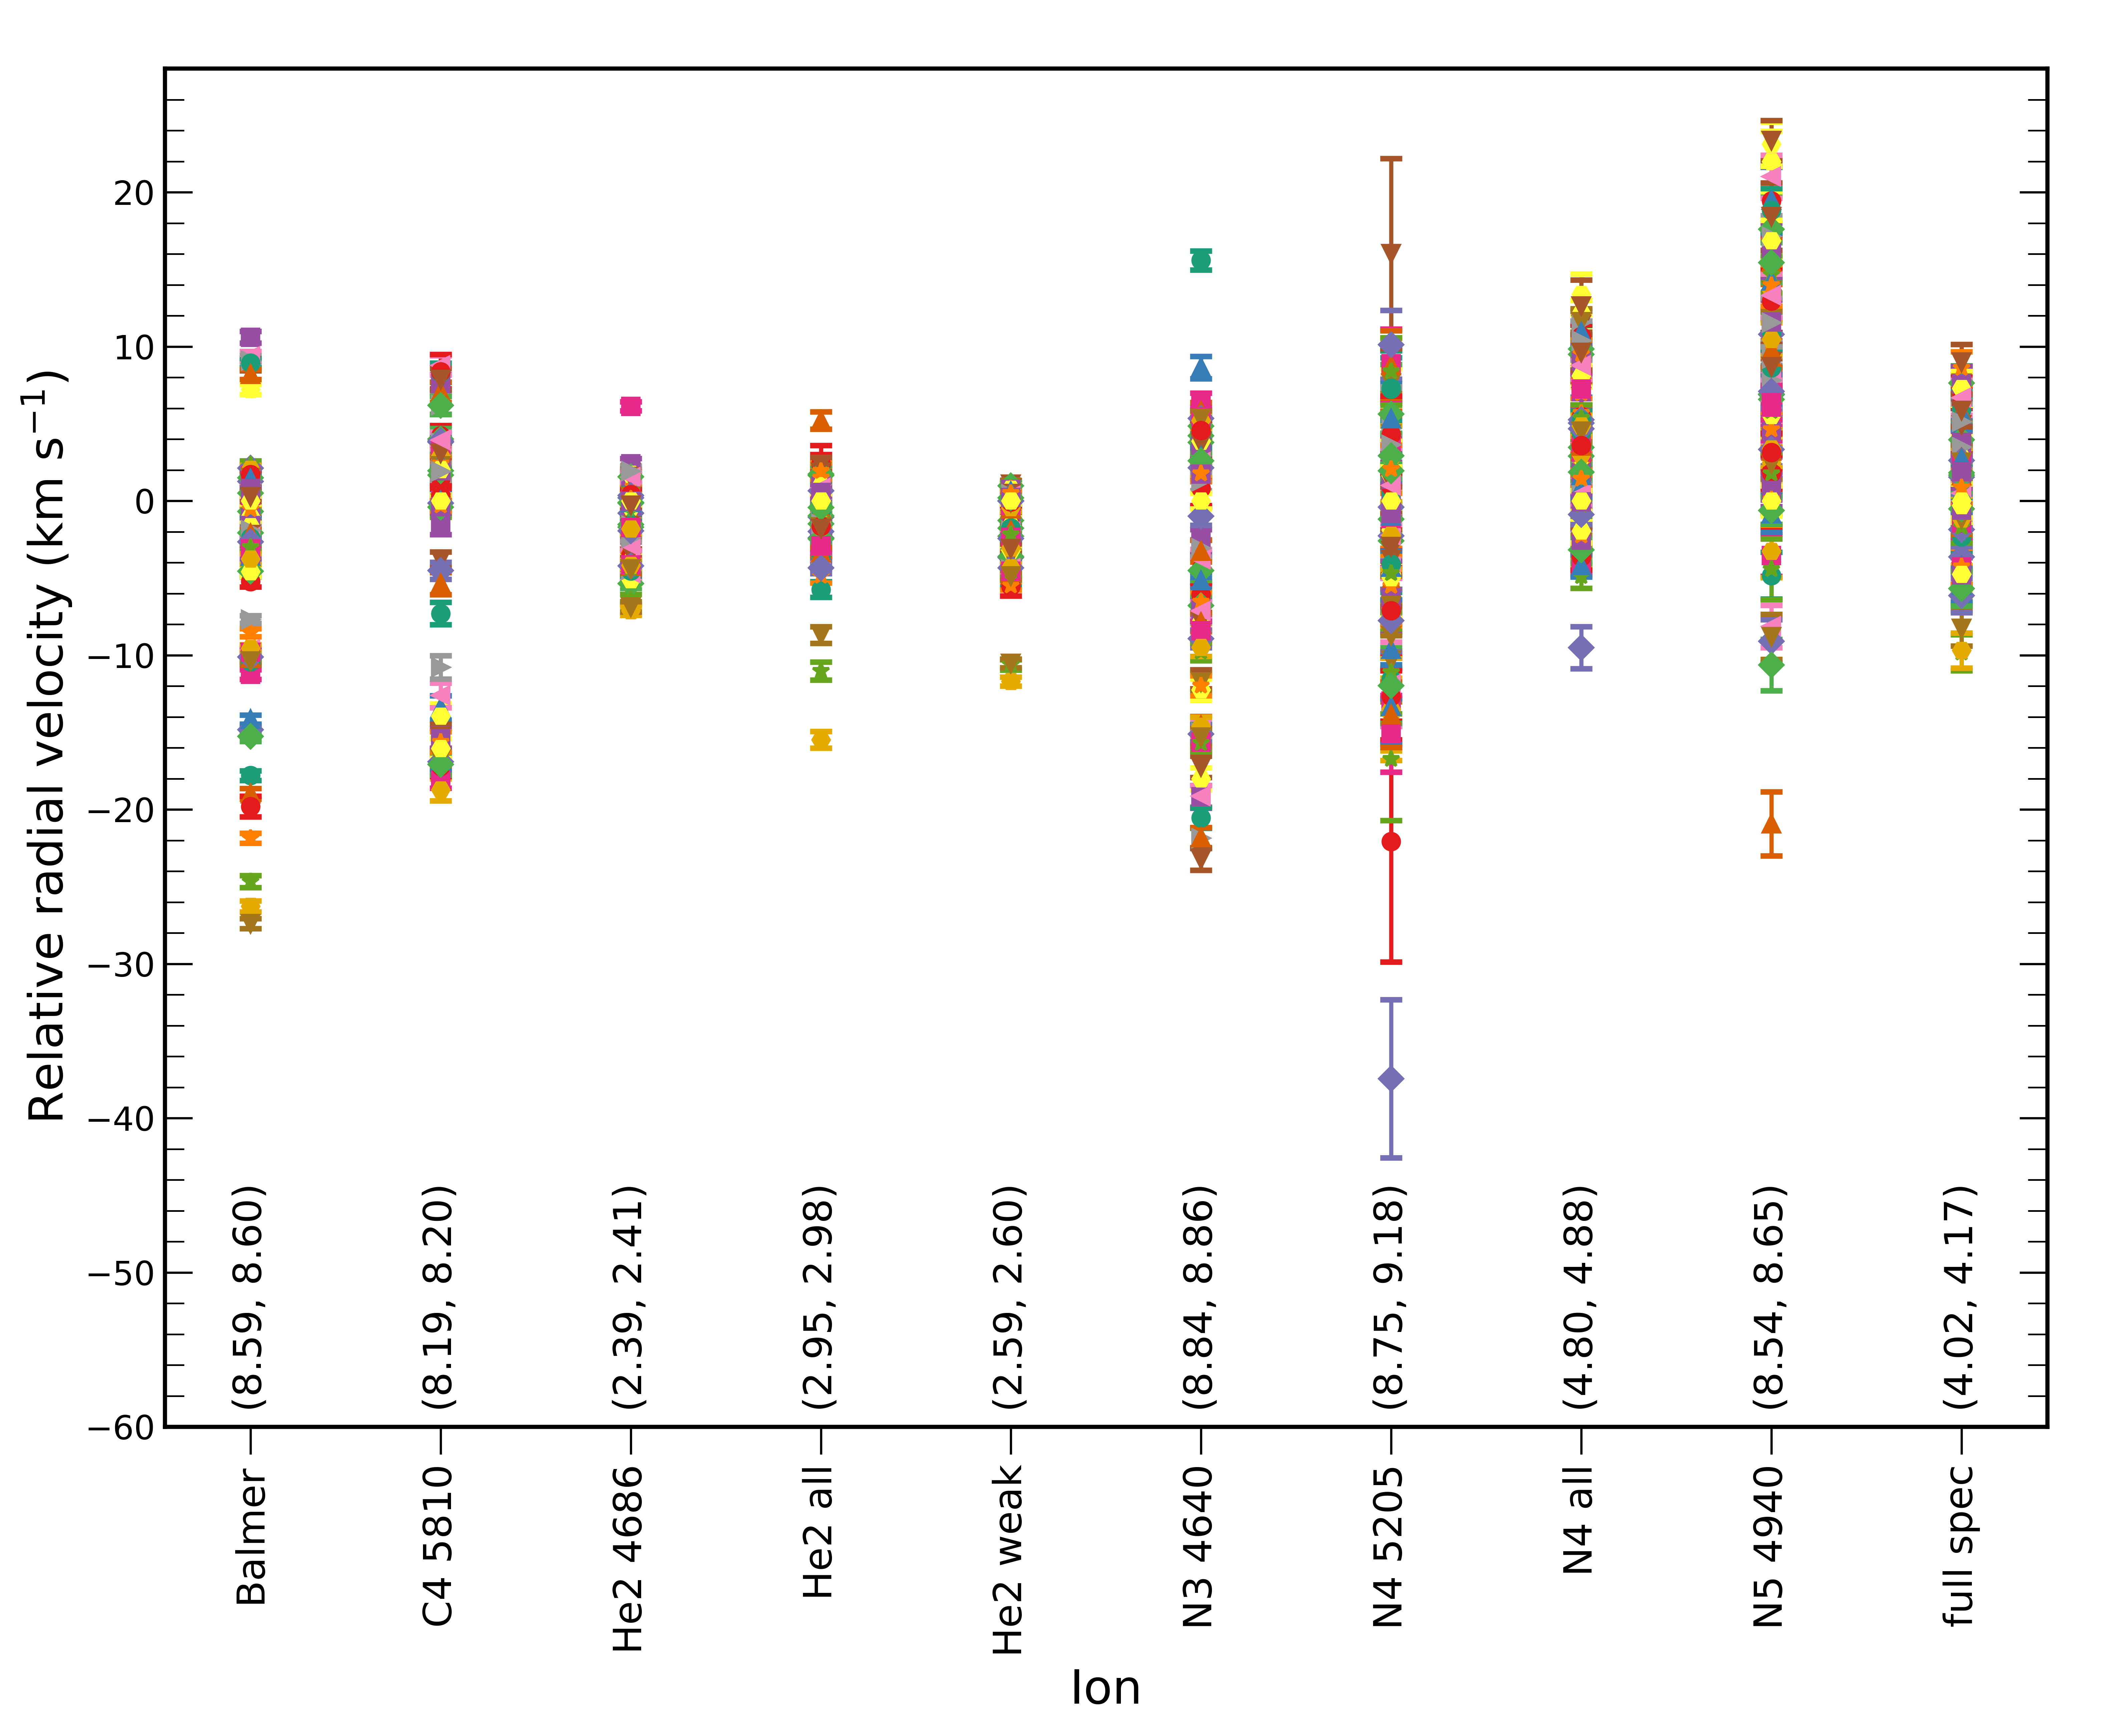
\includegraphics[width=\hsize]{chapters/WNL/image/RV_SC_WR136_ion.png}
    \caption{High-cadence RV measurements for WR 136 over a variety of masks. In brackets at the bottom are values of ($\sigma_w$, \sigRV{}) (\kms{}). As there are 87 data points for each mask, the legend has been omitted for clarity. }
    \label{fig:hc_wr136}
\end{figure}

\label{sect:obsbinfrac}
\begin{figure}
    \centering
    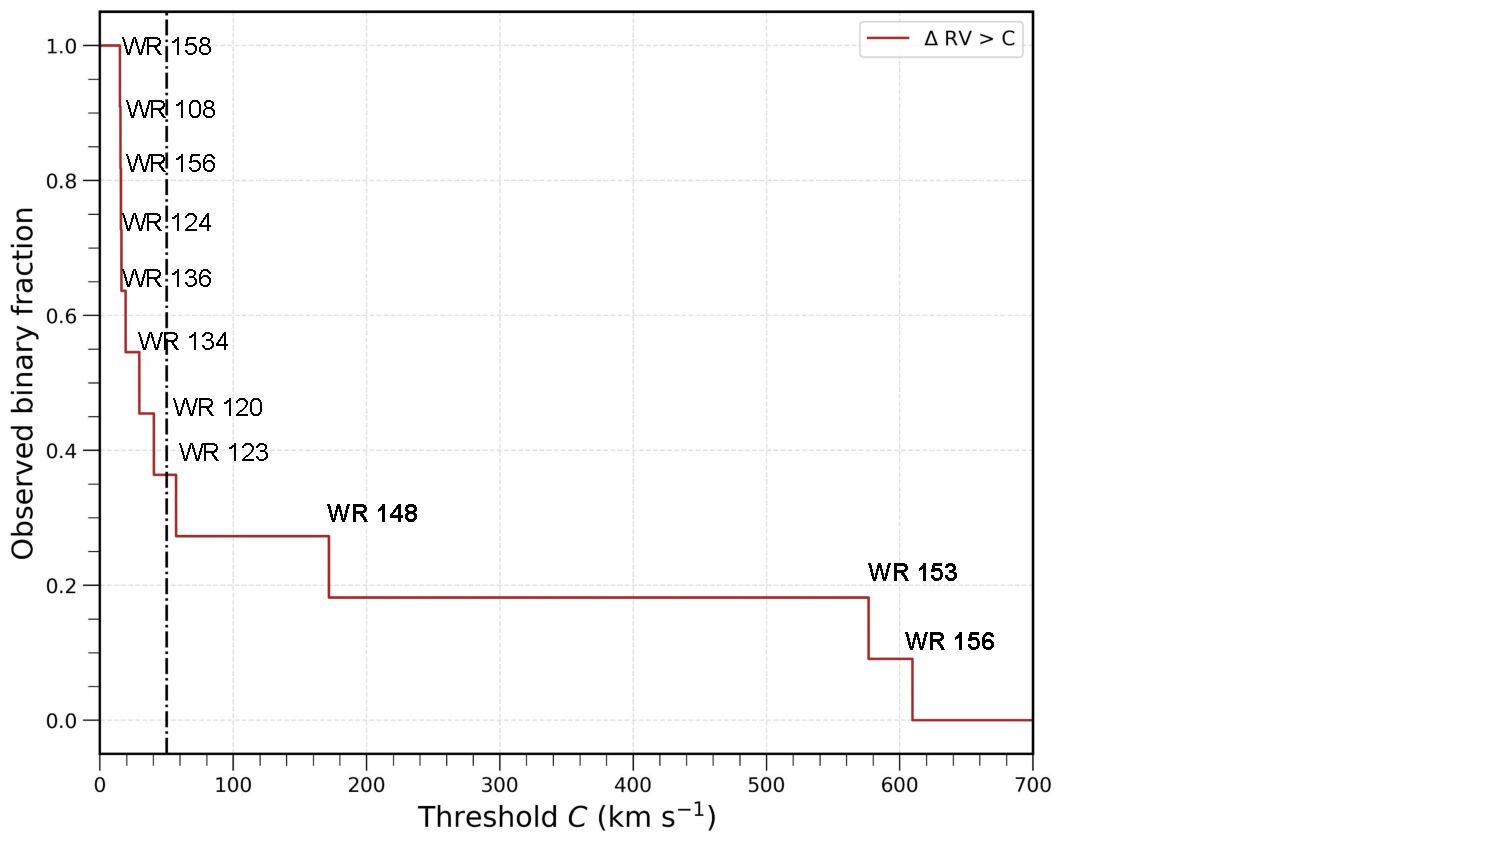
\includegraphics[width=\hsize]{chapters/WNL/image/BINFRAC_WNL_2604.pdf}
    \caption{Non-parametric threshold plot showing the observed binary fraction as a function of the threshold $C$. The adopted threshold of 50\,\kms{} is shown by the dotted-dashed vertical line. The entries in bold are confirmed spectroscopic binaries in the literature.}
    \label{fig:threshold_plot}
\end{figure}

\begin{sidewaystable}
\small
\setlength{\tabcolsep}{0pt}
\centering
\caption{Radial velocity measurements for our sample of WNL stars together with an overview of their known multiplicity properties. $\Delta$ RV and $\sigma_{\textrm{RV}}$ are calculated in this work and are used to identify tentative spectroscopic binaries. The spectral types are taken from the GCWR unless indicated otherwise, with `d.e.l.' implying the dilution of emission lines and `a' indicating the presence of absorption lines. The binary status of this work is reported based on the spectroscopic observations.}

\begin{threeparttable}
% \begin{tabular*}{\textwidth}{ l @{\extracolsep{\fill}} *{8}{d{0.1}} }
\centering
\begin{tabular*}{\textwidth}{l @{\extracolsep{\fill}}*{9}{c}}
% \begin{tabular*}{ccccccccc}
\toprule
\toprule

WR\# & Spectral Type & \multicolumn{2}{c}{Binary Status} & Period & e & $\Delta$ RV  & $\sigma_{\textrm{RV}}$ & \DelRV{} $>$ C\\
 & (GCWR) & (GCWR) & This work & (d) & &(\kms{}) &(\kms{}) &  \\ \midrule
108 & WN9ha & a, d.e.l. & - & - & - & 15.7 & 5.0 & no\\
120 & WN7o & - & - & - & - & 40.5 & 15.7 & no\\
123 & WN8o & SB1?, no d.e.l. & SB & - & - & 57.1 & 18.2 & yes\\
124 & WN8h & SB1?, no d.e.l. & - & - & - & 19.3 & 5.9 & no\\
134 & WN6b & SB1?, no d.e.l. & - & - & - & 29.6 & 9.3 & no\\
136 & WN6b(h) & SB1?, no d.e.l. & - & - & - & 15.4 & 3.0 & no\\
148 & WN8h+ & SB1, d.e.l. & SB & $4.317336\,\pm\,0.000026\,$d\tnote{(a)} & 0 (fixed)\tnote{(a)} & 171.8 & 54.5 & yes\\
153 & WN6o/CE+O3-6 + B0:I+B1:V-III  & SB2\,+\,SB2 & SB & 6.6887\tnote{(b)} & 0.0\tnote{(b)} & 576.6 & 150.3 & yes\\
% 153 & WN6o/CE+O3-6 + B0:I+B1:V-III  & SB2\,+\,SB2 & SB & 6.6887\tnote{(b)}+\,3.4663\,$\pm$\,0.0011  & 0.0\tnote{(b)}+\,0.16\,$\pm$\,0.03 & 576.6 & 150.3 & yes\\
% 153 & \begin{tabular}{@{}c@{}}WN6o/CE+O3-6 \\ + B0:I+B1:V-III\end{tabular}  & SB2\,+\,SB2 & SB & \begin{tabular}{@{}c@{}}6.6887\tnote{(b)} \\ +\,3.4663\,$\pm$\,0.0011\end{tabular}  & \begin{tabular}{@{}c@{}}0.0\tnote{(b)} \\ +\,0.16\,$\pm$\,0.03\end{tabular} & 576.6 & 150.3 & yes\\
155 & WN6o+O9II-Ib & SB2 & SB & 1.6412436\tnote{(c)} & 0.034\,$\pm$\,0.008\tnote{(c)} & 609.5 & 212.0 & yes\\
156 & WN8h & d.e.l. & - & - & - & 16.1 & 4.4 & no\\
158 & WN7h & d.e.l. & - & - & - & 15.0 & 4.1 & no\\3.6 & no\\
\bottomrule
\end{tabular*}
\begin{tablenotes}[para]
    \item[(a)] \citep{munoz_wr_2017},
    \item[(b)] fixed from photometry, \citet{demers_quadruple_2002},
    \item[(c)] \citet{marchenko_wind-wind_1995} fixed period
\end{tablenotes}
\end{threeparttable}
\label{tab:WNL_data}
\end{sidewaystable}

We used lines of \heii{}, \niii{}, \niv{}, \nv{} and Balmer lines to measure RVs for WR 136. The RV dispersion can be seen in Fig. \ref{fig:hc_wr136}. The observed RV dispersion comprises of a statistical part (i.e. the measurement errors, $\sigma_p$) and contribution from wind-variability ($\sigma_w$, see Eq. \ref{eq:sig_RV}). By measuring \sigRV{} and $\sigma_p$, we get an upper limit on the wind variability. For each mask, values of (\sigRV{}, $\sigma_w$) are indicated in Fig. \ref{fig:hc_wr136}. We find that \b{RVs measured using} lines of \heii{} are less affected by wind variability as compared to \NVred{}. One possible reason is that the \NVred{} line is a very weak line in the spectrum of WR 136, limiting its RV accuracy. In any case, the trend of \heii{} lines showing greater stability than lines of nitrogen is unusual, demonstrating that each WR star is unique. The RV amplitudes for the masks are similar to what was found in \citet{koenigsberger_spectral_1980}, although we do not find the same period reported by them after analysing the data with a Lomb-Scargle periodogram \citep{lomb_least-squares_1976,scargle_studies_1982}. \b{Due to the small RV amplitude and lack of coherent periods, we consider WR 136 to be a single star.} We use diagnostic plots such as Fig. \ref{fig:hc_wr136} for each object to select an appropriate mask to measure RVs. These are indicated in Appendices \ref{apdx:comments_WNL} and \ref{apdx:rv_measurements_wnl}.
%__________________________________________________________________
\begin{figure*}[ht]
    \centering
    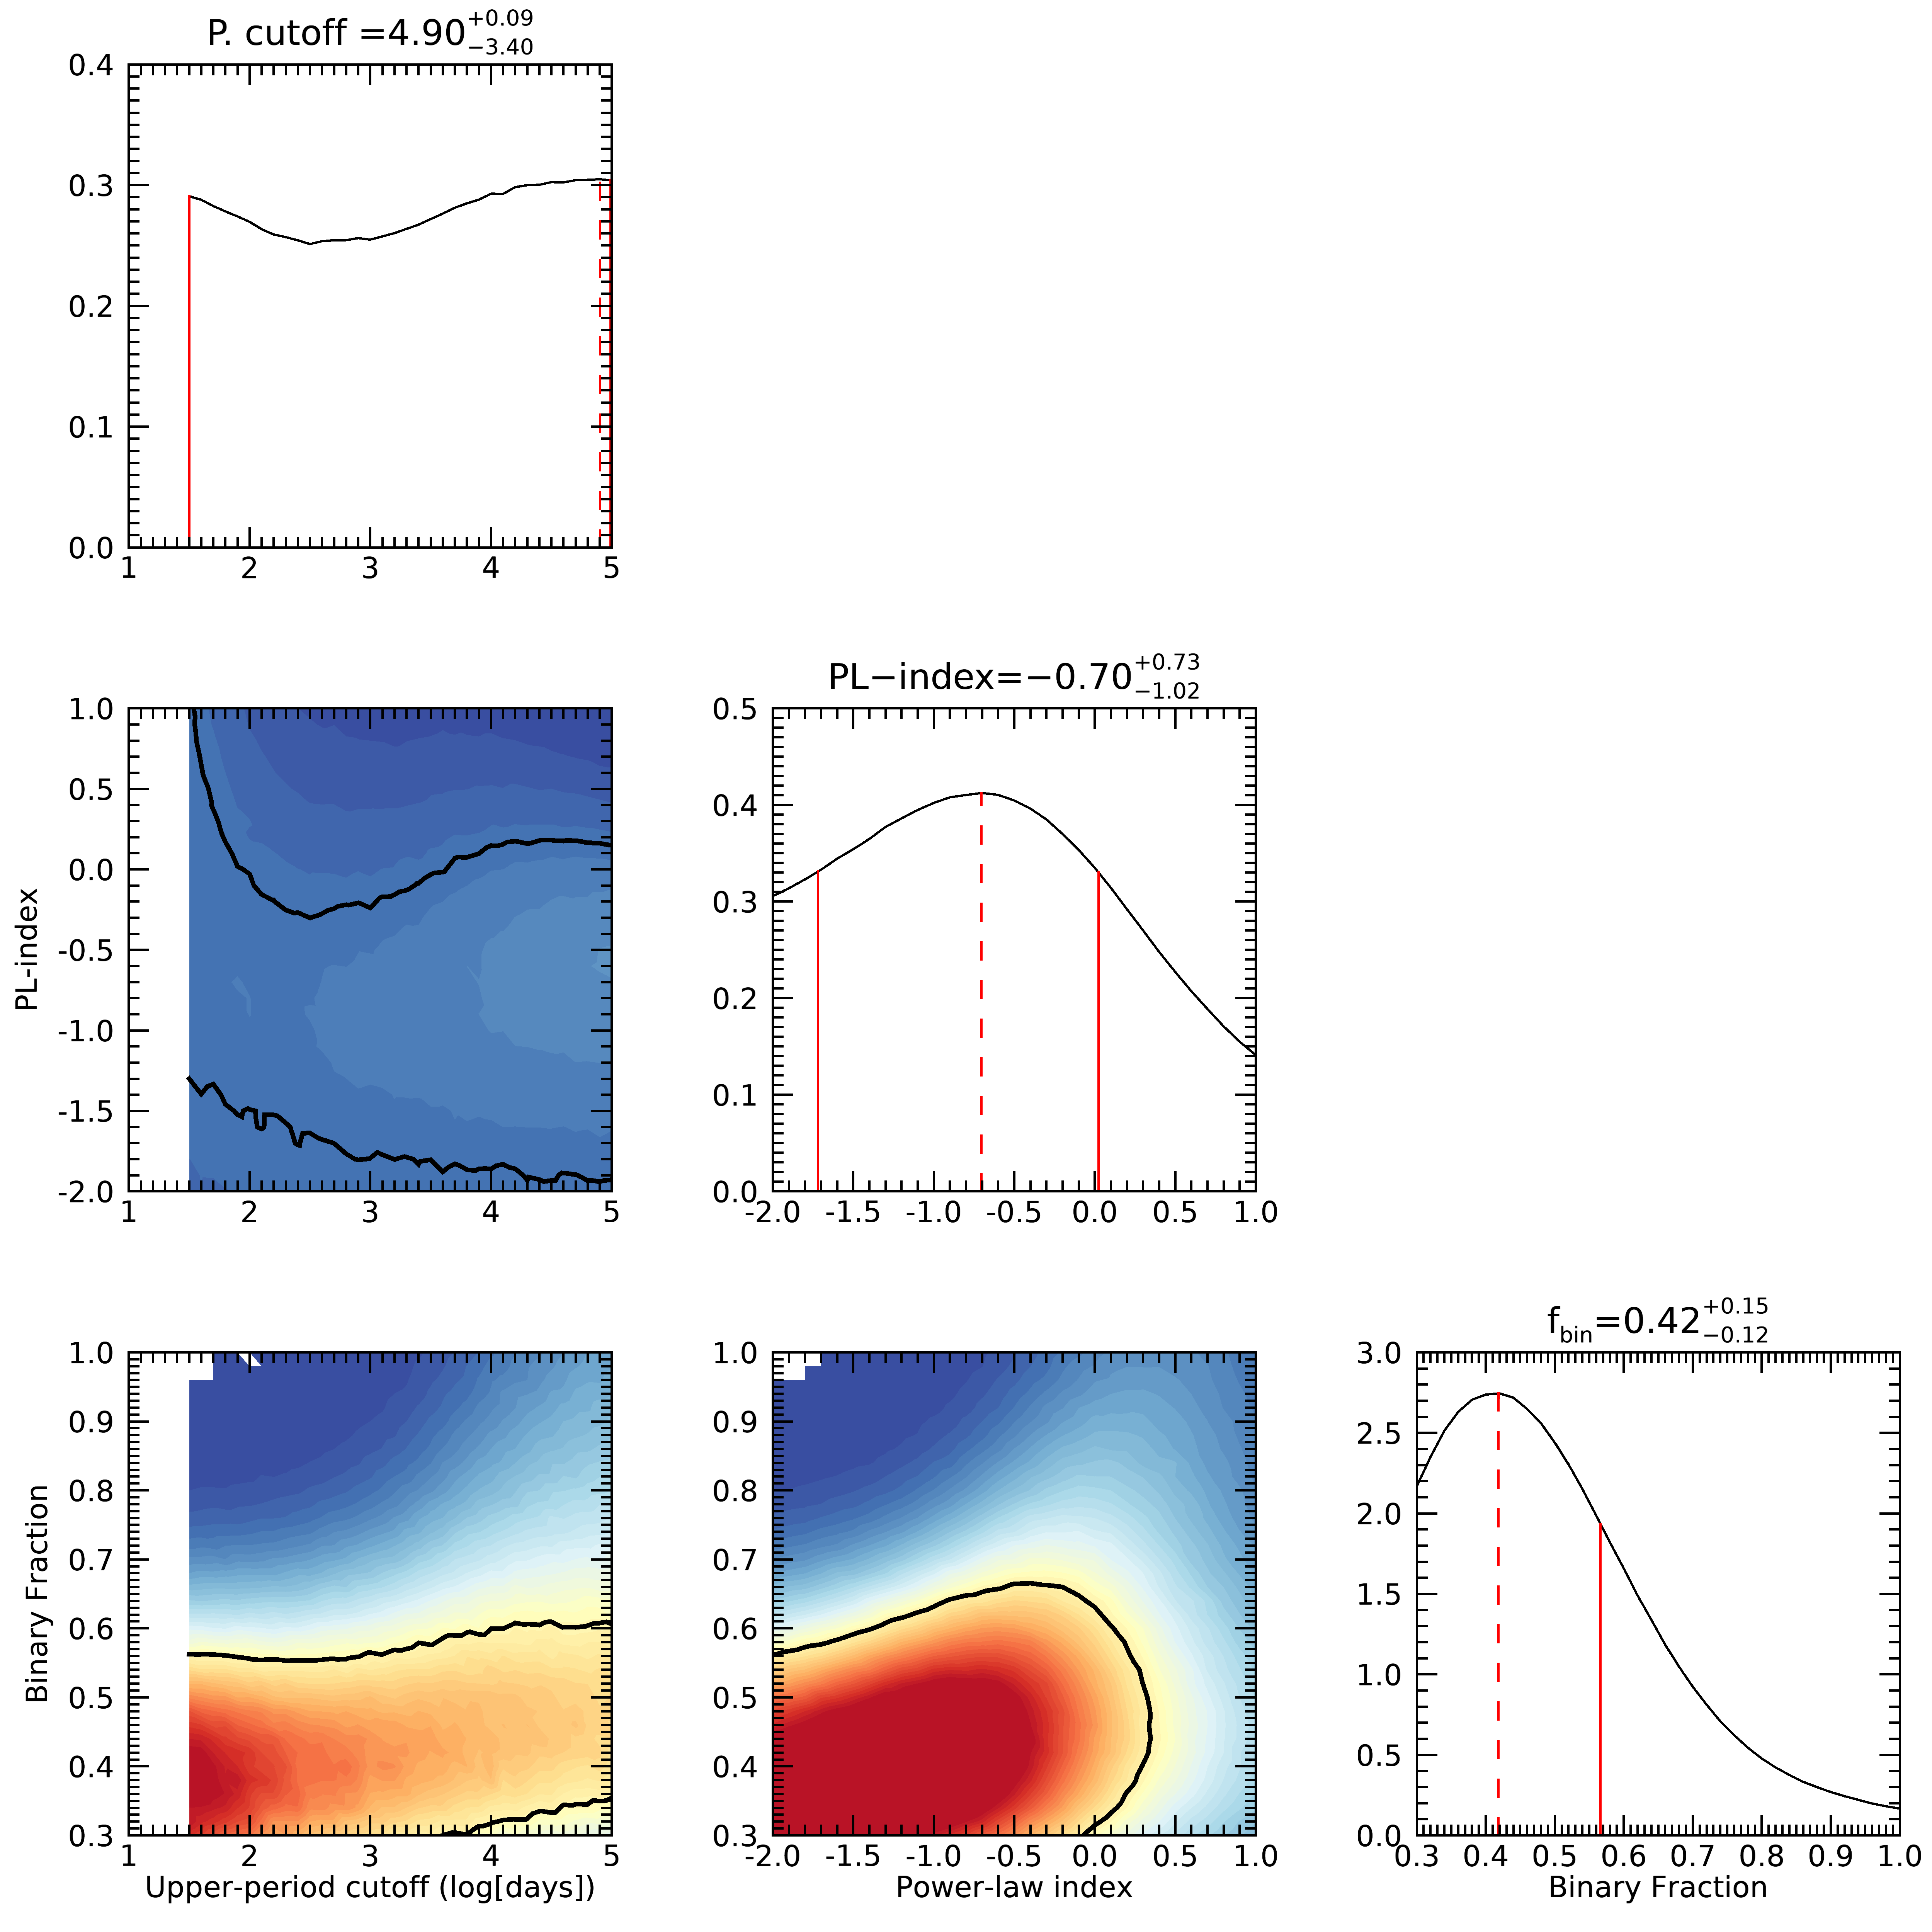
\includegraphics[width=0.85\textwidth]{chapters/WNL/image/WNL_May18_4RVbins_stat9.png}
    \caption{Three-dimensional likelihood over \logPmaxWNL{}, \fintWNL{}, and \piWNL{} for the Galactic WNL population. Assuming flat priors, the one-dimensional posteriors are also shown. For each posterior, the solid red lines show HDI68, and the dashed red line shows the mode.}
    \label{fig:posteriors_WNL}
\end{figure*}


%6.6887\tnote{(b)}\,+\,(3.4663\,$\pm$\,0.0011) & 0.0\tnote{(b)}\,+\,(0.16\,$\pm$\,0.03)

\section{Results} \label{sect:results_WNL}
\subsection{Observed binary fraction and detection probability}
After measuring the RVs, we computed the peak-to-peak amplitude (\DelRV{}) for each object. We chose a threshold $C$ above which we attributed the observed \DelRV{} to Doppler motion in a binary system. Figure \ref{fig:threshold_plot} is a non-parametric threshold plot that shows the observed binary fraction as a function of the chosen threshold. By moving right to left, we attribute the RV amplitude of these stars to Doppler motion, and classify them as candidate spectroscopic binaries.

In principle, the chosen threshold should be high enough to avoid false positives due to intrinsic variability. The high-cadence study on WR 136 demonstrated that with the appropriate mask, the measured peak-to-peak RV amplitude due to intrinsic variability is ${\sim}15$\,\kms{}. This is similar to what was found for the \nv{} lines in WR 138 (Chapter \ref{ch:wc}). Therefore, we adopt a similar strategy and chose a threshold that is at least three times larger than the peak-to-peak intrinsic variability, at $C=50$\,\kms{}. This results in the classification of 4 out of 11 stars as RV variable objects for which binarity is likely the cause. This corresponds to an observed binary fraction (\fobsWNL{}) of 0.36\,$\pm$\,0.15.

%______________________________________________________________
\begin{figure}
    \centering
    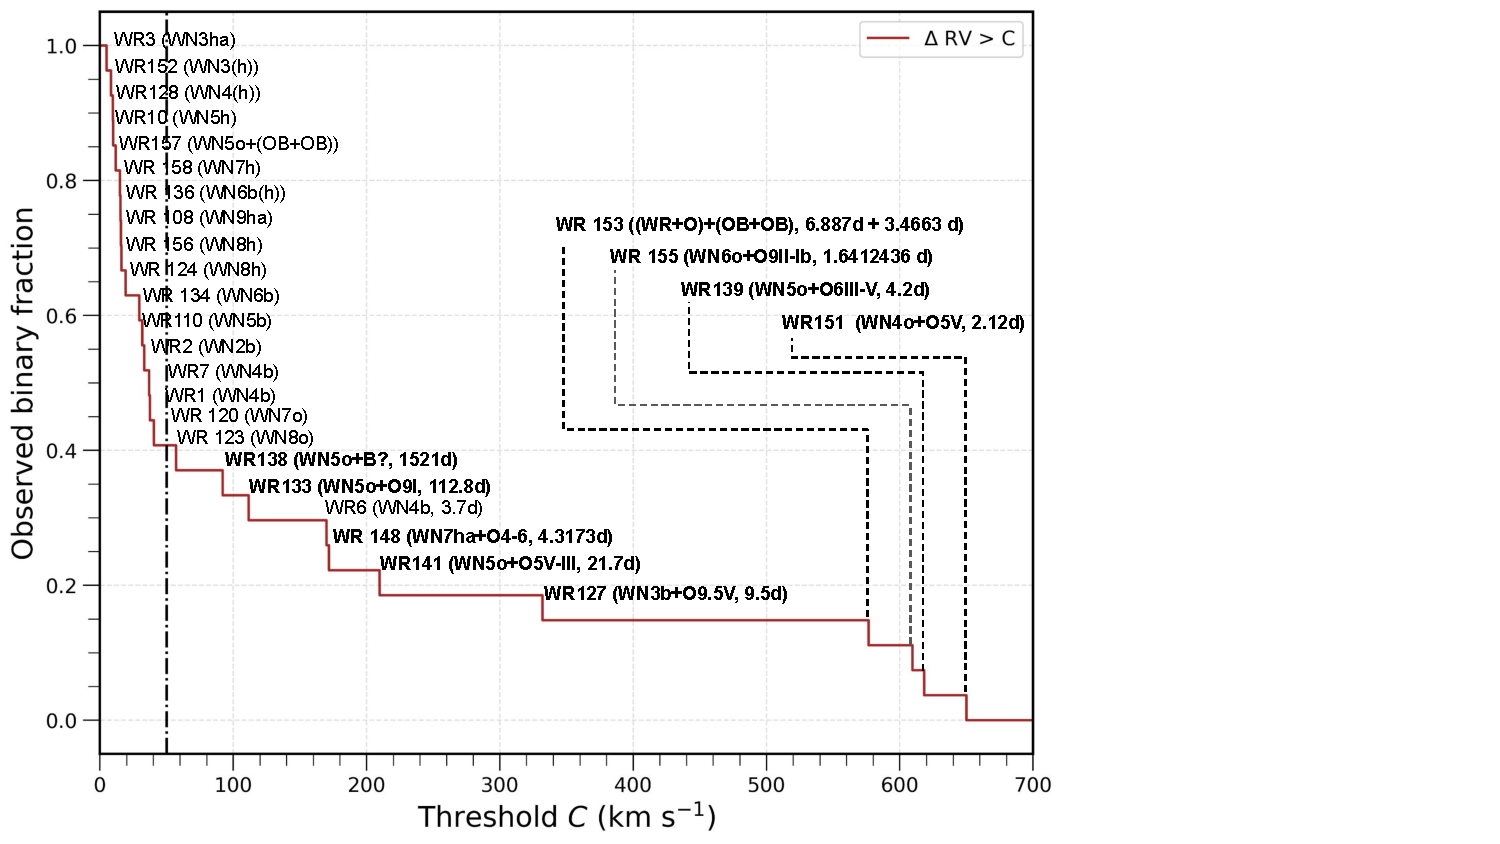
\includegraphics[width=\hsize]{chapters/WNL/image/BINFRAC_WN_1905.pdf}
    \caption{Same as Fig. \ref{fig:threshold_plot} but for the 27 WN stars (16 WNE\,+\,11 WNL) in our sample. The threshold $C=50\,$\kms{} is shown by the vertical dotted-dashed line. Entries in bold represent confirmed spectroscopic binaries in the literature.}
    \label{fig:threshold_plot_WN}
\end{figure}

\begin{figure*}[ht]
    \centering
    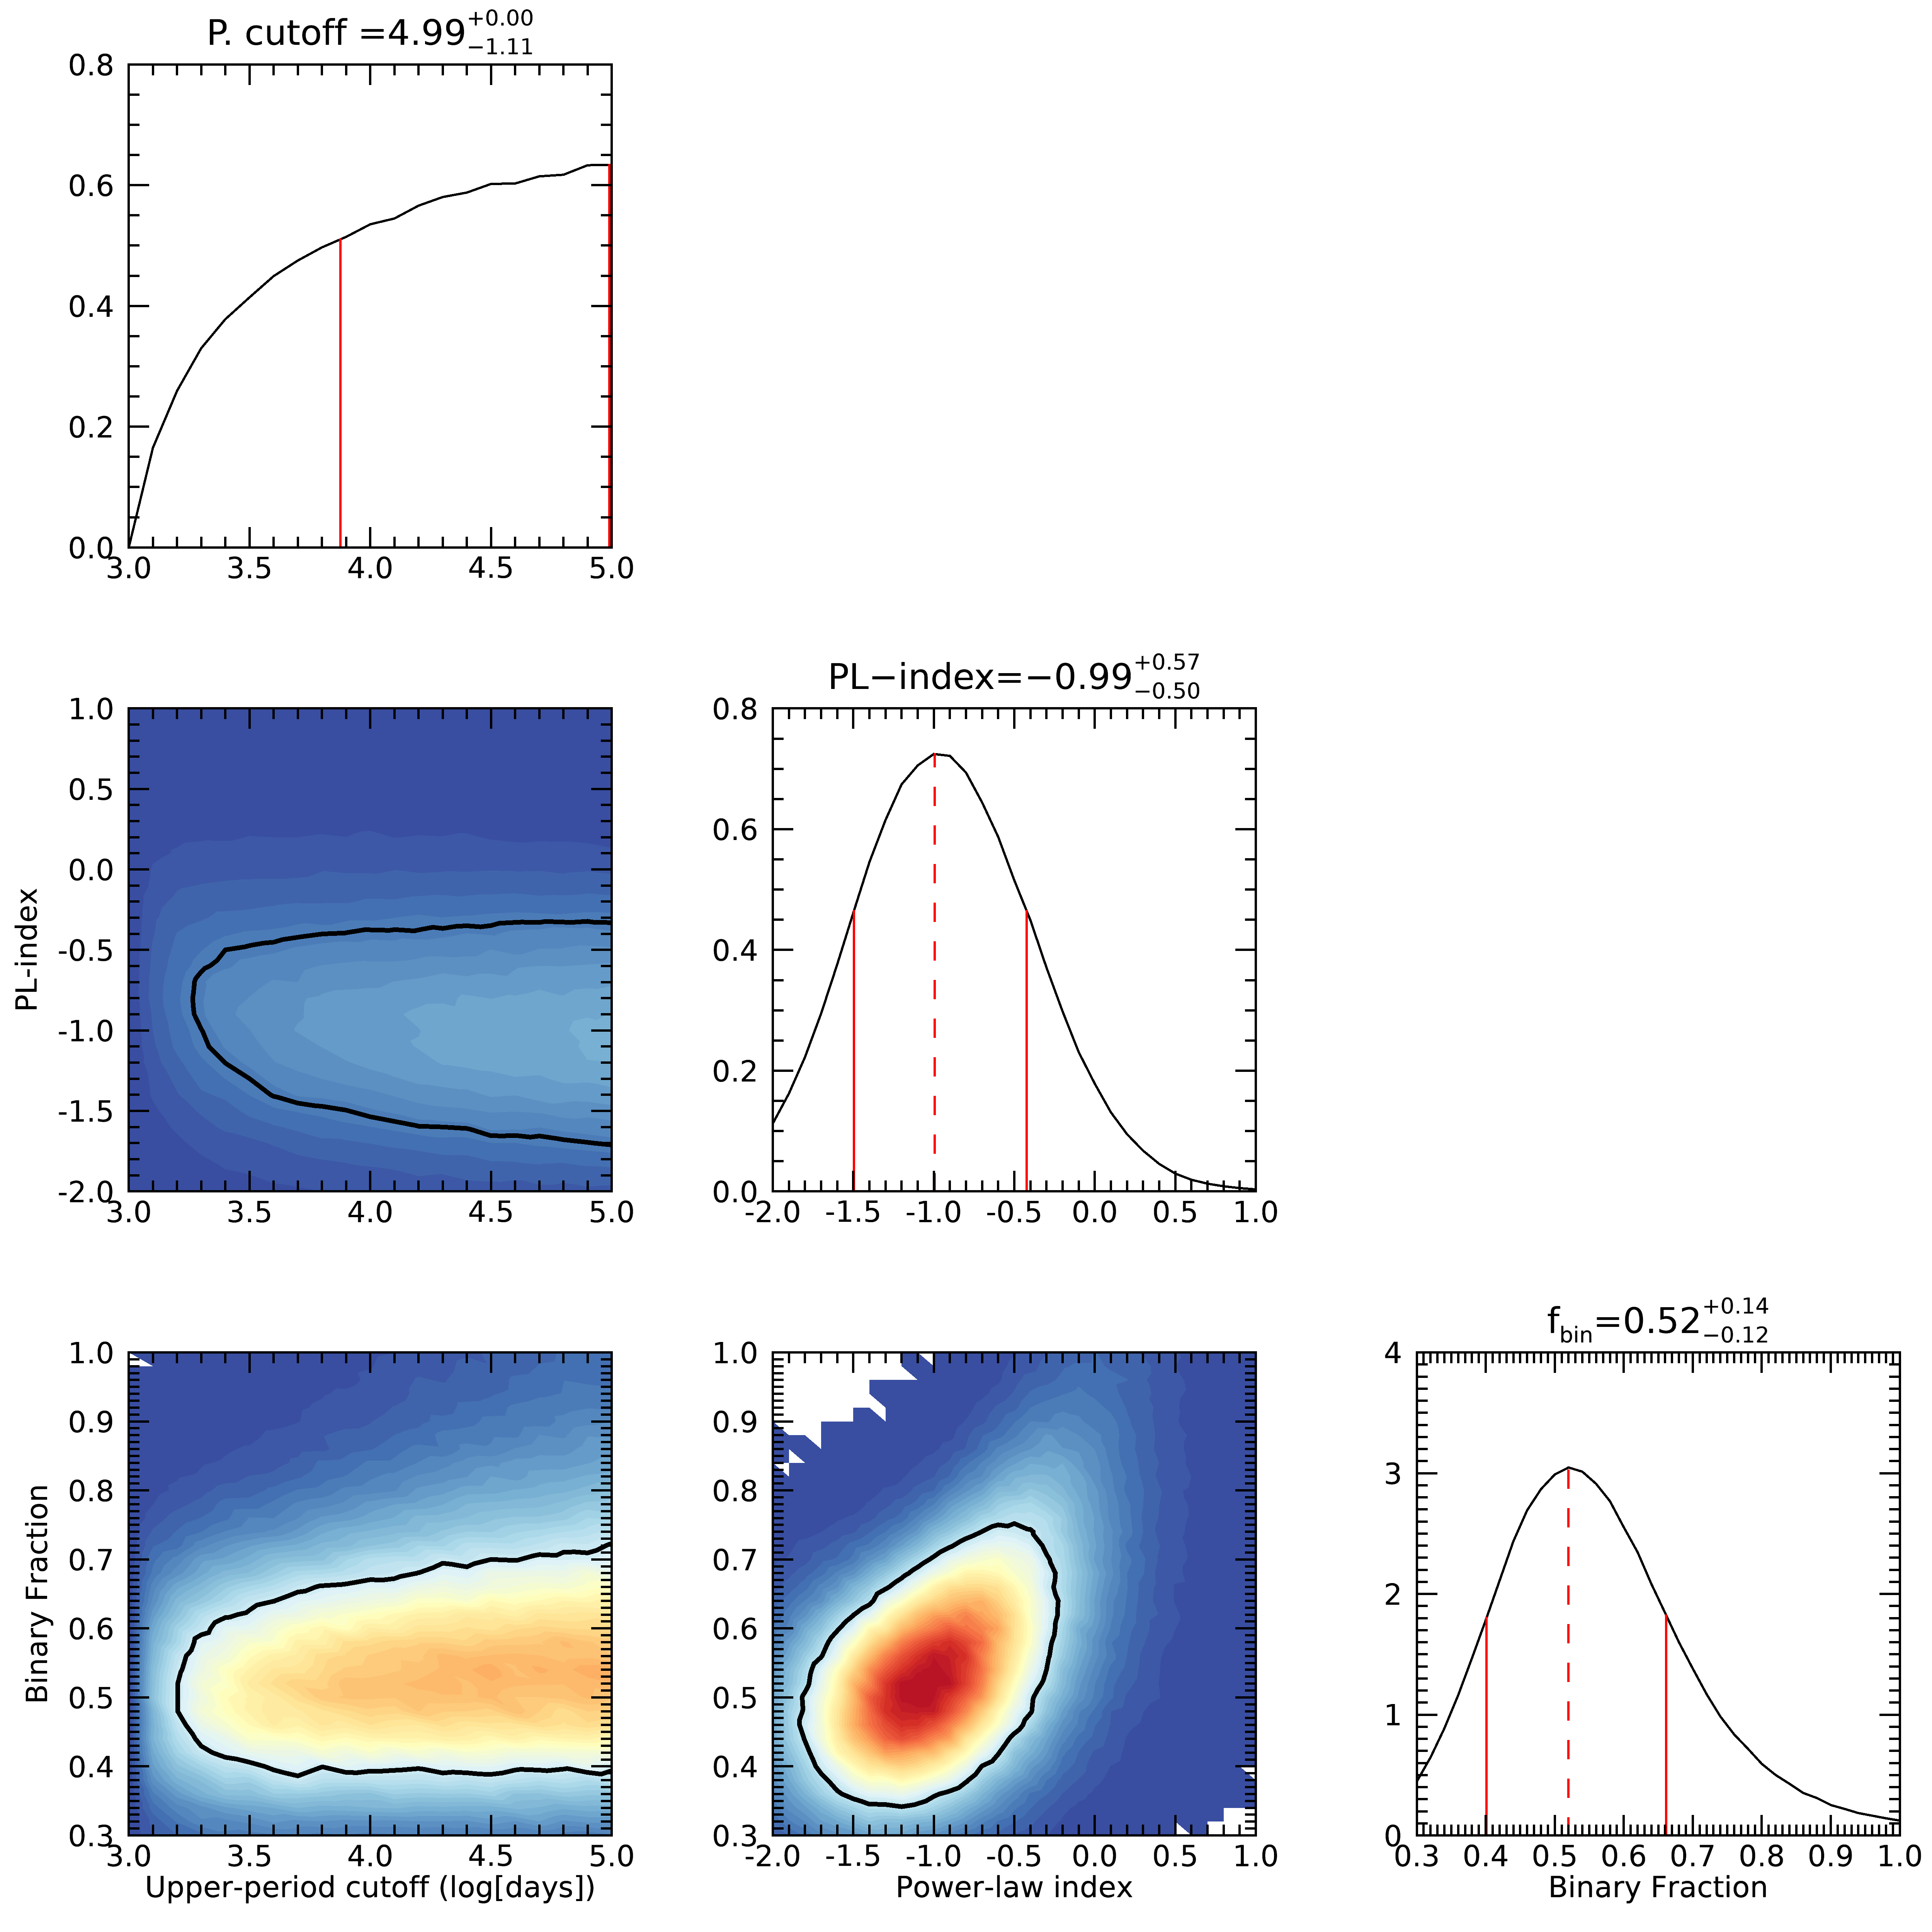
\includegraphics[width=0.85\textwidth]{chapters/WNL/image/WNall_May18_4RVbins_stat9.png}
    \caption{Same as Fig.\,\ref{fig:posteriors_WNL} but for the combined (WNE + WNL) Galactic WN population.}
    \label{fig:posteriors_WN}
\end{figure*}

\begin{figure}
    \centering
    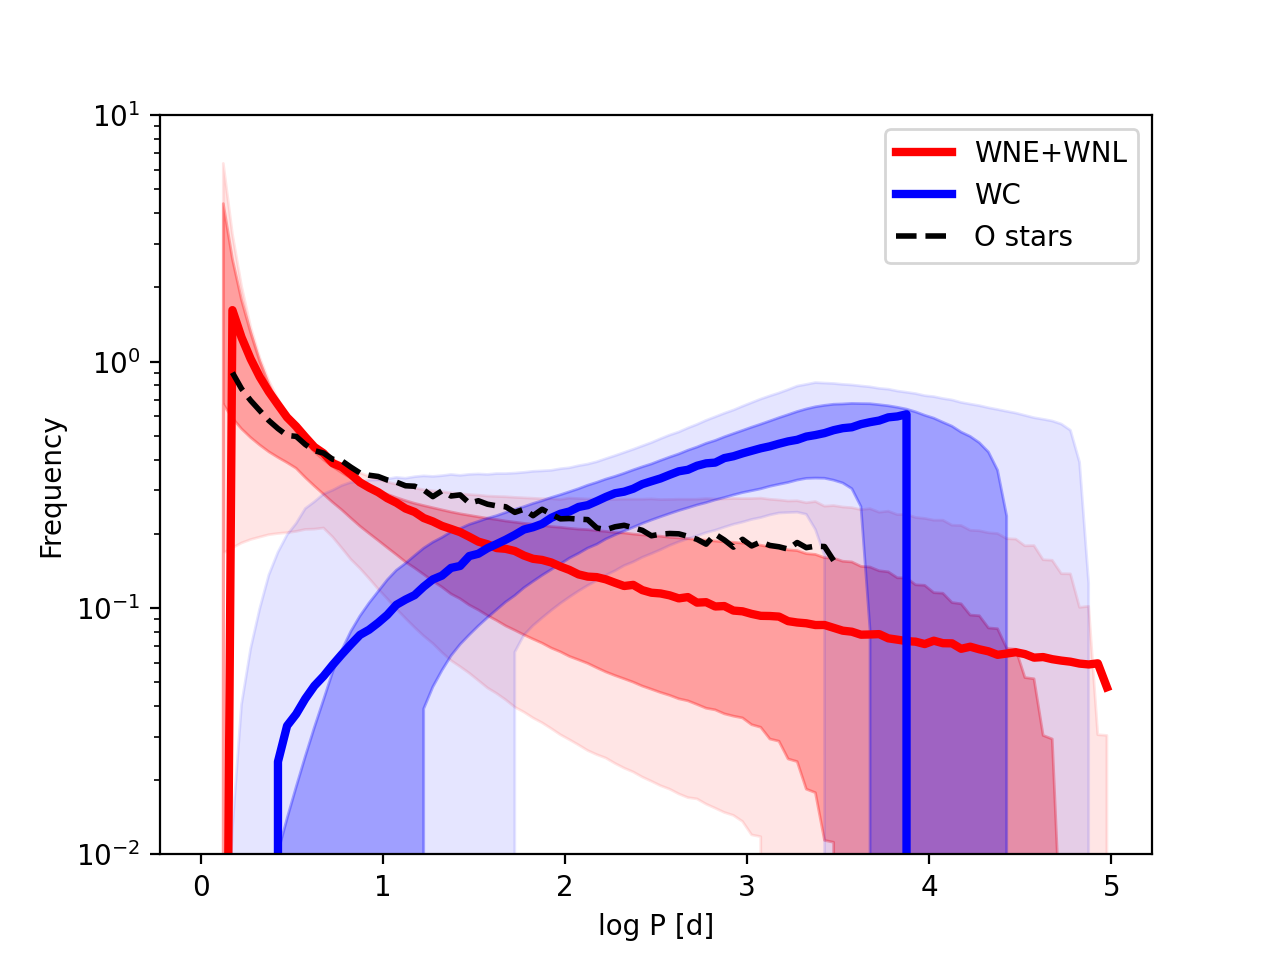
\includegraphics[width=\hsize]{chapters/WNL/image/WNall_sampled_periods_log.png}
    \caption{Visualisation of the $10^7$ period distributions created by sampling the posteriors from Fig.\,\ref{fig:posteriors_WN}. The light- and dark-red regions depict 95\% and 68\% of all distributions. The solid red line is the distribution created with the best-fit values from the posteriors. The blue regions and lines are the same for the WC population from Chapter \ref{ch:wne}. The dashed black line is the period distribution for O stars from \citet{sana_binary_2012}.}
    \label{fig:pdist_WN_WC}
\end{figure}
\subsection{Multiplicity properties: WNL population} \label{sect:WNL_multiplicity}

We perform a Bayesian analysis with MC simulations with a method developed in Chapter \ref{ch:wne} to formally account for the observational biases. The ideal solution is to calculate the likelihood of the observed RV time series for each object based on the sampling and possible binary properties of the system. However, this is too computationally intensive, and instead we divide the objects into multiple \DelRV{} bins and try to reproduce them with our simulations. The \DelRV{} bins are: \DelRV{}\,$<$\,50\,\kms{} (7 objects), $50\,\le\,$\DelRV{}$\,<\,250\,$\kms{} (2 objects), $250\,\le\,$\DelRV{}$\,<\,650\,$\kms{} (2 objects), \DelRV{}\,$\ge\,650\,$\kms{} (no objects).

The parameters included in the model for the population with binaries are the period distribution, intrinsic binary fraction, inclination, eccentricity, mass ratio, time of periastron passage and the orientation of the binary system in three-dimensional space. The period distribution is characterised by the minimum period (\logPminWNL{}), maximum period (\logPmaxWNL) and the power-law index (\piWNL{}). The power-law index $\pi$ determines the shape of the distribution of binaries with orbital periods $P$ as follows

\begin{equation}
    p(\log P) \sim (\log P)^{\pi}.
\end{equation}

Along with the period distribution, we include the intrinsic binary fraction, \fintWNL{}, as a model parameter. The eccentricities are drawn from a flat distribution between 0.0 and 0.9, with random inclinations, times of periastron passage and three-dimensional orientations of the orbital planes. Given the presence of very short-period binaries in the WNL sample, we fixed the value of \logPminWNL{} at 0.15 [d] (approximately 1\,d). We explored values of \logPmaxWNL{} from 1.5 to 5.0 [d] in steps of 0.1 dex, \piWNL{} from $-2.0$ to $1.0$ in steps of 0.1 and \fintWNL{} from 0.30 to 1.00 in steps of 0.02. We also use prior information on the known orbital periods for those classified as binaries (Table \ref{tab:WNL_data}), and require at least three objects with $1<P<10\,$d.

With the framework set up, we simulated 10\,000 sets of 11 WNL stars for each $P-M_2$ grid point, resulting in almost $4 \times 10^8$ populations. We calculated the three dimensional likelihood of reproducing the observed distribution of objects in \DelRV{} bins. Assuming flat priors on \logPmaxWNL{}, \piWNL{} and \fintWNL{}, we computed their marginalised posterior likelihoods (Fig. \ref{fig:posteriors_WNL}). We computed the 68\% credible intervals for each posterior (the highest density interval, HDI68). For the three model parameters, our posteriors yield values of \fintWNL{}$\,=\,0.42\substack{+0.15 \\ -0.12}$, \piWNL{}$\,=\,-0.70\substack{+0.73 \\ -1.02}$ and \logPmaxWNL$\,=\,4.90\substack{+0.09 \\ -3.40}\,$ [d] for the parent WNL population. The value of \logPmaxWNL{} is set by the upper limit of the grid due to the lack of long-period constraints introduced by the orbital bins, as a result of no confirmed WNL binaries at $P>10\,$d.

The derived multiplicity properties are in agreement with those of the Galactic WNE population (Chapter \ref{ch:wne}). An interesting difference is that of the upper-period cutoff, which is better constrained for the WNE population (\logPmaxWNE{}\,$= 4.60\substack{0.40 \\ -0.77}$) given the prior information on the presence of long-period binaries. We do not have such constraints for the WNL population, with the only orbital periods that are constrained in the literature are less than 10 days (Table \ref{tab:WNL_data}). This results in a large HDI68 for \logPmaxWNL{}, which is reconcilable with \logPmaxWNE{} within the credible intervals.

The negative power law index for the WNL sample indicates a preference for binary systems with shorter orbital periods. This is similar to what was found for the WNE (Chapter \ref{ch:wne}) and O-type populations \citep{sana_binary_2012}. The lower cut off for the orbital period distribution (\logPminWNL{}) is fixed at 0.15 [d] in order to account for the presence of binaries with periods as short as 1.6\,d in our sample. The similarities with respect to the WNE population are indicative that the overall multiplicity properties of the Galactic WN population are consistent. We therefore combine the WNE and WNL populations and perform a similar Bayesian analysis.
%______________________________________________________________


\subsection{Multiplicity properties: combined WN population}  \label{sect:WN_multiplicity}
After merging the data sets of the 16 WNE stars in Chapter \ref{ch:wne} and the 11 WNL stars in this paper, we ended up with 27 Galactic WN stars. Based on their \DelRV{} values, we created Fig. \ref{fig:threshold_plot_WN}, similar to Fig. \ref{fig:threshold_plot}, depicting \fobsWN{} as a function of the threshold $C$. The characteristic kink in the curve can be seen around 50\,\kms{}, differentiating RV variation due to Doppler motion and intrinsic variability, thereby reaffirming our choice of threshold. We therefore constrained the observed binary fraction for the WN sample to be \fobsWN{}\,$=\,0.41$\,$\pm$\,$0.09$.

We performed a Bayesian analysis on the combined WN sample with the same underlying assumptions for the distributions stated in Sect. \ref{sect:WNL_multiplicity}. We divided the sample into various \DelRV{} bins as follows: \DelRV{}\,$< 50\,$\kms{} (16 objects), 50\,$\le$\,\DelRV{}\,$<250\,$\kms{} (6 objects), 250\,$\le$\,\DelRV{}\,$<650$ (6 objects), \DelRV{}\,$\ge\,650$\,\kms{} (no objects). Similarly, we also defined minimum orbital period bins based on what is known for the sample: $P\,>\,1\,$d (10 objects), $P\,>\,10\,$d (3 objects), $P\,>\,100\,$d (2 objects) and $P\,>\,1000\,$d (1 object). The three-dimensional likelihood, along with the one-dimensional posteriors computed by assuming flat priors are shown in Fig.\,\ref{fig:posteriors_WN}. As compared to Fig.\,\ref{fig:posteriors_WNL}, the power-law index (\piWN{}) becomes more negative and \fintWN{} on the WN population increases due to the contribution from the WNE sample.

The derived multiplicity properties for the WN sample were used to construct a visualisation of the period distribution. Similar to Chapter \ref{ch:wne}, we sampled $10^7$ sets of parameters from the posteriors in Fig.\,\ref{fig:posteriors_WN} and used them to create orbital period distributions. The density cloud representing these distributions can be seen in red in Fig.\,\ref{fig:pdist_WN_WC}. The period distribution constructed using the best-fit parameters is shown with a solid red line. We also plotted the density cloud of distributions for the Galactic WC population in blue (Chapter \ref{ch:wne}). The period distribution for main-sequence O stars is shown with a dashed-black line \citep{sana_binary_2012}.
%______________________________________________________________
\begin{figure}
    \centering
    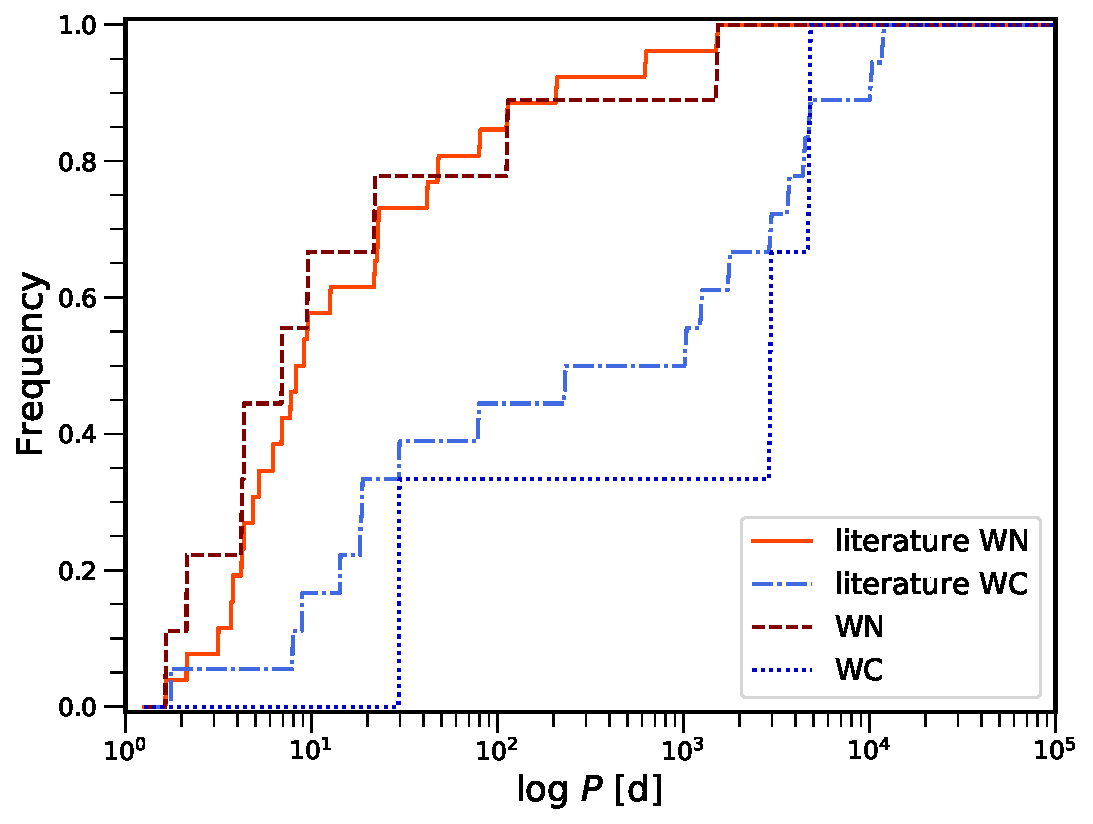
\includegraphics[width=\hsize]{chapters/WNL/image/Cumulative_pobs_with_HERMES.pdf}
    \caption{Cumulative distribution of the reported orbital periods from the literature for the Galactic WN (solid red) and WC (dashed-dotted blue) populations. The observed distributions based on spectroscopic periods from our sample are also plotted, with the WN (dashed red) and WC (dotted blue) binaries.}
    \label{fig:obs_pdist_WNL}
\end{figure}
\section{Discussion} \label{sect:discussion_WNL}
\subsection{Comparison with the literature}  \label{sect:lit}
In order to verify if what is observed is in agreement with our results, we investigated the literature to consider WR stars beyond those included our sample. Since the objects from \citetalias{van_der_hucht_viith_2001} have been thoroughly analysed for binarity, we focus on this subset of WR stars. The catalogue contains 87 WC stars and 127 WN stars, of which 78 are WNL stars. Of these 78 objects, 21 are classified as spectroscopic binaries and 14 currently have orbital solutions. Of these, only one has a period larger than 100 days.

The total number of Galactic WN binaries with known orbital periods is 28. Combining this with the 18 known orbital periods for Galactic WC binaries, we constructed the cumulative observed orbital period distribution with the distribution from our sample over-plotted (Fig.\,\ref{fig:obs_pdist_WNL}). While a few WC binaries have periods shorter than 10\,d, this fraction is still much smaller than that of short-period WN binaries. This shows that the analysed samples are representative of the Galactic WR population.
%______________________________________________________________
% \subsection{Comparison with the WNE and WC samples}  \label{sect:WNEandWC}
%______________________________________________________________
\subsection{Observational biases due to the limiting magnitude}  \label{sect:mag}
Another potential observational bias introduced by the conditions of the RV campaign is that of the limiting magnitude. Because WR stars are generally faint in the optical, the selection criteria of $V\le12$ inherently favours binaries. \citet{vanbeveren_binary_1980} demonstrated this clearly for the Large Magellanic Cloud, although this effect is not dominant in the Galaxy due to the large spread in the distances.

Similar to what was done in Chapter \ref{ch:wne}, we assumed that the companion contributes to around 50\% of the flux in WR\,$+$\,OB system \citep[e.g.,][]{shenar_wolf-rayet_2019}. Therefore, WR binaries would be twice as bright as single WR stars on average. To account for this bias, we need to account for single WR stars between 12.0 and 12.7 mag. In cases where the $V$-band magnitude was missing, we searched for $\varv$-band magnitudes between 13.0 and 13.7.

We found five single WNL entries in that range: WR\,58 (WN4b/CE), WR\,63 (WN7o\,$+$\,OB), WR\,82 (WN7(h)), WR\,130 (WN8(h)), and WR\,131 (WN7h+abs). Although WR\,63 and WR\,131 could be considered candidate binaries, no evidence of a companion has been found in the literature, and hence we conservatively consider them to be single stars. Including these stars in our sample would change the intrinsic binary statistics, from 5 binaries out of 11 WNL stars to 5 binaries out of 16 WNL stars. This would result in a binary fraction of 0.31, which is within our credible interval.
%______________________________________________________________
\subsection{Consequences on binary evolution}  \label{sect:orbitalprop}
Depending on their mass, main-sequence O stars are thought to evolve into either red supergiants or luminous blue variables (LBVs) before becoming WR stars, after which they are expected to collapse to form compact objects \citep{1976Conti,meynet_stellar_2003,crowther_physical_2007,langer_presupernova_2012}. In this section, we use our derived multiplicity properties for the Galactic WN and WC populations to infer possible connections between the evolutionary stages before collapse. As the multiplicity properties of the WNL and WNE populations are compatible, we discuss the WN population as a whole.

% The Conti scenario hypothesises that as single O stars strip their outer envelopes via their strong stellar winds, their spectral appearance evolves to WN, WC, and WO (if massive enough) before they collapse to form a compact object (preferentially a black hole). However, the majority of O stars live their lives in interacting binaries and the impact of binary evolution is not well constrained.

\subsubsection{Linking the O and WN populations}\label{sect:OWN}

As indicated in Fig.\,\ref{fig:pdist_WN_WC}, the orbital period distributions of O stars and WN stars is in excellent agreement. This is not surprising, given that WN stars can be formed by the envelope stripping of the primary by the secondary in an OB binary. Using the analytical expressions from \citet{soberman_stability_1997}, it is possible to calculate the change in the orbital period due to mass transfer. Depending on the mass-ratio of the OB binary, mass transfer does not increase the orbital period by more than a factor of three, irrespective of the mass-ratio and the conditions for mass transfer. For example, conservative mass transfer in a 40\,$+$\,30\,\Msun{} binary where the primary transfers 20\,\Msun{} would have an increase in the period ($P_f/P_i$) of factor 1.7. Therefore, the increase in the orbital period would not shift the distribution drastically, which is in accordance with what we find.

A possible exception where binary interaction can significantly reduce the orbital period is common envelope evolution, triggered by mass transfer in systems with extreme mass ratios or after the donor has developed a deep convective envelope (see, e.g. the review by \citealt{ivanova_common_2013}). However, envelope ejection is energetically disfavored unless interaction happens after the star becomes a red supergiant \citep[e.g.][]{klencki_it_2021}, but this phase is potentially not reached by the most massive stars as it would require evolution beyond the Humphreys-Davidson limit \citep{humphreys_studies_1979,davies_luminosities_2018,gilkis_excess_2021}.

Depending on their initial mass, massive stars are also thought to go through the LBV phase during their transition from main sequence O stars to the WN phase. Multiplicity studies on the LBV population indicate a binary fraction of 0.70\,$\pm$\,0.09, with the majority of them at periods of a year or longer \citep{mahy_multiplicity_2022}. The multiplicity properties of the LBVs seem inconsistent with the large number of short period WN binaries that is found both in our sample and in the GCWR (Fig.\,\ref{fig:obs_pdist_WNL}). However, this could just be a consequence of shorter period systems being too compact to fit an LBV star, leading an O star to fill its Roche lobe before reaching that evolutionary phase. This would imply that the progeny of the LBV binary population are the WN binaries with $P>1$\,yr.

\subsubsection{Evolution from the WN to WC populations}\label{sect:evol_WNWC}

The biggest discrepancy between the orbital period distributions for both the observed (Fig.\,\ref{fig:obs_pdist_WNL}) and intrinsic (Fig.\,\ref{fig:pdist_WN_WC}) populations is the glaring lack of WC binaries at short periods. Because WN stars are expected to evolve into WC stars by further stripping their envelope, the change in their orbital parameters is governed by wind or binary mass loss. This results in an increase of the orbital period by a factor of ${\sim}1.5$-2. Therefore, this implies that only WN binaries with $P>100\,$d would preferentially evolve into WC binaries. In the short period regime of $P<10\,$d, only a small fraction of WN binaries might become WC binaries.

One possibility for WNE stars in short period binaries to avoid evolving into WC binaries requires that they are unable to strip their envelopes further before reaching core collapse, for example, due to reduced mass loss rates \citep[possible implications from][]{neijssel_wind_2021}. Why would this only affect WN binaries with short periods and not the entire population is unclear. Another possibility is that short period WN binary systems undergo interaction before they can reach the WC phase. The cause of this interaction could potentially be the expansion of the WN star due to inflation \citep{grafener_stellar_2012,sanyal_massive_2015,grassitelli_subsonic_2018,ro_wolf-rayet_2019}. While it is unclear if inflation happens in nature, and how an inflated donor star would respond to mass transfer, an unstable mass transfer phase resulting in a merger could prevent short period WN stars from evolving into WC binaries. Conversely, if such mass transfer episodes are stable, they would result in further stripping, leading to more short period WC stars and worsening the discrepancy in the period distributions.

Additionally, in systems undergoing wind-wind collisions, slowed outflows may potentially interact with the binary and be ejected with additional angular momentum, leading to a contraction of the orbit and possibly a merger. For example, \citet{macleod_pre-common-envelope_2020} showed how the interaction of colliding winds with the stars in equal mass main sequence binaries could lead to a shrinkage of the orbit. Depending on the ratio of the orbital velocity to the wind velocity, this effect could also occur to WN binaries. Whether this scenario provides a valid explanation remains to be shown.

A final possible scenario could be that the O star companion fills its Roche lobe before the WN evolves into a WC, but the likelihood of it happening during the short-lived WNE phase is too small for this to be the predominant explanation for the lack of short period WC systems.

Due to the duration and sampling of the RV campaign, it is also possible that there is a population of long-period binaries ($P>1000\,$d) that we do not detect. This is because the intrinsic variability of WN stars is larger than that of the WC, making it challenging to detect low RV amplitudes. Therefore, it could be that the progenitor population of long-period WC binaries is simply undetected. However, this would imply that for the Galactic WN population the value of \fintWN{} is close to 1.00, as most (all?) the apparently single WN stars would then reside in long-period binary systems.

% \subsection{Higher-order systems}

A large fraction of the main sequence O population are in hierarchical triple systems \citep[e.g.,][]{sana_southern_2014,moe_mind_2017}. Mass loss due to stellar winds or binary stripping, among other things, will cause the ratio of the inner and outer separation to change. If the stripping of the primary by the secondary resulted in a WN\,$+$\,OB binary, then the nature of mass transfer and evolution of the inner orbit determines the stability of the triple. When this ratio changes beyond a critical point, the system becomes dynamically unstable. This could result in the disruption of the triple, or a merger of the inner binary \citep{toonen_evolution_2020}.

In the case of mass loss through stellar winds, the dynamically unstable phase can last from thousands to millions of years \citep{toonen_stellar_2022}. Although the most common outcome predicted is the preservation of the triple hierarchy, it is also common for the system to be disrupted with one of the stars ejected. In case of an ejection, the resulting orbit has a period of the order of $10^3$-$10^5\,$d \citep{toonen_stellar_2022}. As an example in a hierarchical triple, if the inner WN\,$+$\,OB binary was formed through a combination of stripping via stellar winds and mass transfer, it could be dynamically unstable. An ejection could result in the formation of a WN\,$+$\,OB binary in a wide orbit, where the WN star would go on to evolve and become a wide WC\,$+$\,OB binary. Detailed simulations involving the formation of the WR star, mass transfer and stellar winds are required to investigate the frequency and feasibility of this channel.

% When scrutinising the population of WNE binaries, their further evolution also raises questions. According to the Conti scenario, WNE stars evolve into WC stars if enough mass is shed. From Fig. \ref{fig:periodDistShift}, we can see that there is a lack of WC binaries with periods below 20\,d compared to the WNE and O star populations. The orbital evolution from the WNE to the WC phase is mainly governed by mass loss due to their stellar winds which will widen the orbit, so a shift to longer periods is expected.
%______________________________________________________________
\section{Conclusions} \label{sect:conclusions_WNL}
With a homogeneous, magnitude-limited spectroscopic monitoring of 11 northern Galactic WNL stars, we measured relative RVs using cross-correlation and found \fobsWNL{}\,$=0.36\,\pm\,0.15$. Using a Bayesian framework around MC simulations, we derived a fraction corrected for observational biases (\fintWNL{}$\,=\,0.62\substack{+0.16 \\ -0.17}$). We observed that the computed intrinsic multiplicity properties for the Galactic WNL population are congruous with those derived for the WNE population in Chapter \ref{ch:wne}.

%as: \fintWNL{}$\,=\,0.62\substack{+0.16 \\ -0.17}$, \piWNL{}$\,=\,-0.6\substack{+0.8 \\ -0.9}$ and \logPmaxWNL$\,=\,1.9\substack{+1.9 \\ -0.4}$. This is

We combined the WNE and WNL samples and simulated ${\sim}15\,\times\,10^9$ populations of 27 WN stars. We found the intrinsic multiplicity properties for the Galactic WN population to be similar to those derived for main-sequence O stars in \citet{sana_binary_2012}. We constructed the orbital period distribution for Galactic WNs and noted the peak at $P<5\,$d. The abundance of short period WN binaries can be explained through Case A or Case B mass transfer in O binaries. Short-period WN binaries can also form via common envelope evolution through late Case B or Case C mass transfer, irrespective of the mass-ratio. However, it is observationally non-trivial to distinguish between the multitude of channels.

From the intrinsic multiplicity properties of the Galactic WC population (Chapter \ref{ch:wc}), we see a clear lack of short-period WC binaries, with the orbital period distribution peaking at $P\,{\sim}\,5000\,$d. The lack of short-period WC binaries is also supported by the literature. While there are a few known, their number is lacking compared to their WN counterparts, despite the fact that the number of WNs and WCs in the Galaxy are similar. The discrepancy in distributions is not only found in our simulations (Fig.\,\ref{fig:pdist_WN_WC}) but can also be seen in the observed period distribution of Galactic WR binaries (Fig.\,\ref{fig:obs_pdist_WNL}). Orbital evolution via mass loss from the WN to WC phase cannot explain the shift towards longer periods.

The multiplicity properties of Galactic LBVs \citep{mahy_multiplicity_2022} seems to be in agreement with that of the long-period O, WN and WC binary populations. This could imply that, at long periods, the evolutionary channel of O$\,\xrightarrow{}$\,LBV\,$\xrightarrow{}$\,WN\,$\xrightarrow{}$\,WC might exist. However, the evolution of the short-period WN binaries is still an enigma. Invoking exotic channels such as common-envelope evolution and dynamical interactions in triples could explain their evolution, but they are highly uncertain. Further observational and theoretical studies are required to understand their importance in the grand scheme of binary evolution.

As the immediate progenitors of black holes, the multiplicity properties of WR stars directly affect those for black hole binaries (e.g. through black-hole kicks in a core-collapse scenario), and hence the predictions for gravitational-wave progenitors. Expanding the sample size of magnitude-limited studies is critical to understand the binary evolution of massive stars.
